\documentclass[11pt,a4paper]{report}

\usepackage{float} %dzieki temu pakietowi rysunki pojawiaja sie tam gdzie chce po uzyciu opcji H w srodowisku figure
\usepackage[font=small,labelfont=bf]{caption}
\usepackage{natbib}
\usepackage{import}
\usepackage[tight]{subfigure}
\usepackage{tikz}
\usepackage{pgfplots}
\usepackage{polski}
\usepackage[cp1250]{inputenc}
\usepackage{indentfirst}
\usepackage{color}
\usepackage{graphics}
\usepackage{geometry}
% ---- PAGE LAYOUT ----
\geometry{a4paper, top=1.5cm, bottom=1.5cm, left=1.5cm,
right=1.5cm, nohead}
\usepackage{amsmath,amssymb,amsfonts}
\begin{document}
\begin{center}
\large{\textbf{PRACA DOMOWA I}}
\end{center}

\noindent
imi� i nazwisko ........................................\\


\noindent
\textbf{Zadanie 1} :\\
\textbf{(a)} 1) Wyznacz dziedzin� funkcji $f(x) = \ln\frac{x}{1-x^2}$, 2) Wyznacz dziedzin� funkcji, r�wnania asymptot, naszkicuj wykres funkcji  $f(x) =  \frac{2x+3}{4x-3}$,\\
\textbf{(b)} 1) Wyznacz dziedzin� funkcji $f(x) = \sqrt{x^3-6 x-4}$, 2) Wyznacz dziedzin� funkcji, r�wnania asymptot, naszkicuj wykres funkcji  $f(x) = \frac{x^2+1}{2 x-3}$,\\
\textbf{(c)} 1) Wyznacz dziedzin� funkcji $f(x) = \sqrt{\frac{3}{x^2}+\frac{2}{x+1}-\frac{3}{x}}$, 2) Wyznacz dziedzin� funkcji, r�wnania asymptot, naszkicuj wykres funkcji  $f(x) = \frac{2 x^2+1}{x^2-4}$,\\
\textbf{(d)} 1) Wyznacz dziedzin� funkcji $f(x) = \ln \left(-\frac{5}{x+3}+\frac{1}{x+1}+\frac{6}{(x+1)^2}\right)$, 
2) Wyznacz dziedzin� funkcji, r�wnania asymptot, naszkicuj wykres funkcji  $f(x) = \frac{x^3-x^2-1}{9-x^2}$.\\

\vspace{0.25cm}

\noindent\textbf{odpowiedzi}:\\ 
\textbf{(a)}\\ 
1) $x \in (-\infty,-1)\cup (0,1)$,\\ 
2) $x\in \mathbb{R}\setminus\left\{\frac 34\right\}$, $\lim\limits_{x\rightarrow \frac{3}{4}^{-}} f(x) = -\infty,\ 
\lim\limits_{x\rightarrow \frac{3}{4}^{+}} f(x) = +\infty$, 
$\lim\limits_{x\rightarrow -\infty} f(x) = \lim\limits_{x\rightarrow +\infty} f(x) = \frac 12$,\\ 
asymptoty: pionowa $x = \frac 34$, pozioma $y = \frac 12$
\\
\textbf{(b)}\\ 
1) $x\in \langle -2, 1 - \sqrt{3} \rangle \cup \langle 1 + \sqrt{3}, +\infty )$,\\ 
2) $x\in \mathbb{R}\setminus\left\{\frac 32\right\}$, 
$\lim\limits_{x\rightarrow \frac{3}{2}^{-}} f(x) = -\infty,\ 
\lim\limits_{x\rightarrow \frac{3}{2}^{+}} f(x) = +\infty$,\\
asymptota pionowa: $x = \frac 32$, asymptota uko�na $y = \frac 12 x + \frac 34$,\\ 
$\lim\limits_{x\rightarrow -\infty} f(x)/x = \lim\limits_{x\rightarrow +\infty} f(x)/x = \frac 12$, 
$\lim\limits_{x\rightarrow -\infty} (f(x)-x/2) = \lim\limits_{x\rightarrow +\infty} (f(x)-x/2) = \frac 34$
\\
\textbf{(c)}\\
1) $x\in (-\infty,-\sqrt{3}\rangle \cup \langle -1,0) \cup (0,\sqrt{3}\rangle$,\\ 
2) $x\in \mathbb{R}\setminus\left\{-2,2\right\}$, $\lim\limits_{x\rightarrow -2^{-}} f(x) = +\infty,\ 
\lim\limits_{x\rightarrow -2^{+}} f(x) = -\infty,$  
$\lim\limits_{x\rightarrow 2^{-}} f(x) = -\infty,\ 
\lim\limits_{x\rightarrow 2^{+}} f(x) = +\infty$,\\
$\lim\limits_{x\rightarrow -\infty} f(x) = \lim\limits_{x\rightarrow +\infty} f(x) = 2$, asymptoty: pionowe $x = -2$, $x = 2$, pozioma $y = 2$\\
\textbf{(d)}\\
1) $x\in (-\infty, -3) \cup (-2,-1) \cup (-1,2)$, \\
2) $x\in \mathbb{R}\setminus\left\{-3,3\right\}$, 
$\lim\limits_{x\rightarrow -3^{-}} f(x) = +\infty,\ 
\lim\limits_{x\rightarrow -3^{+}} f(x) = -\infty,$  
$\lim\limits_{x\rightarrow 3^{-}} f(x) = +\infty,\ 
\lim\limits_{x\rightarrow 3^{+}} f(x) = -\infty$,\\
asymptoty pionowe: $x = -3,\ x = 3$, asymptota uko�na $y = -x + 1$,\\ 
$\lim\limits_{x\rightarrow -\infty} f(x)/x = \lim\limits_{x\rightarrow +\infty} f(x)/x = -1$, 
$\lim\limits_{x\rightarrow -\infty} (f(x)+x) = \lim\limits_{x\rightarrow +\infty} (f(x)+x) = 1$

\begin{figure}[H]
	\centering
	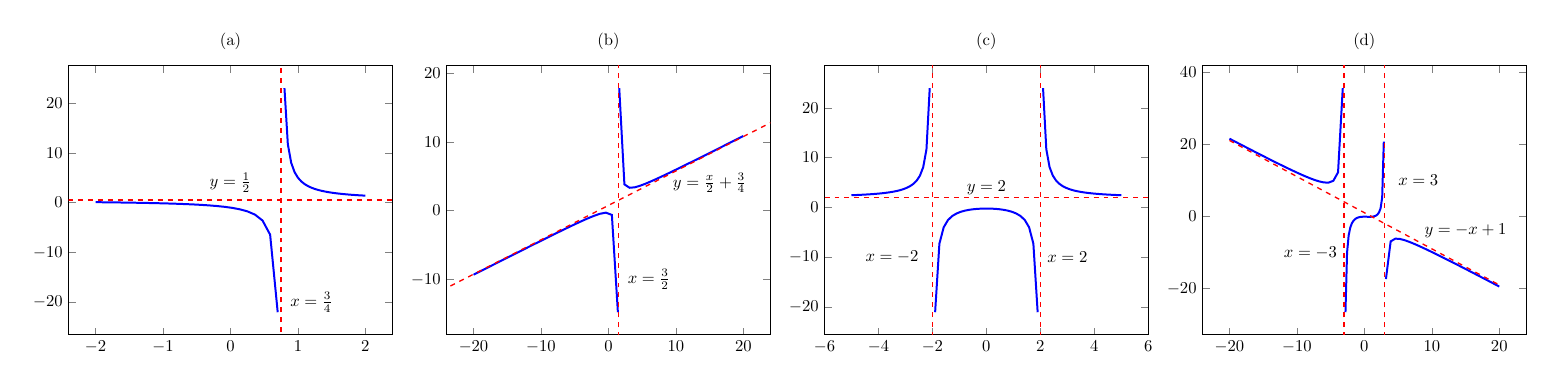
\begin{tikzpicture}[scale=0.6]
		\begin{axis}[title = {(a)}]
			\addplot[domain=-2:0.7,blue,very thick] {(2*x+3)/(4*x-3)};
			\addplot[domain=0.8:2,blue,very thick] {(2*x+3)/(4*x-3)};
			\draw[dashed,red,thick] (axis cs: 0.75,-30)--(axis cs: 0.75,30);
			\draw (axis cs: 1.2,-20) node {$x = \frac 34$};
			\draw[dashed,red,thick] (axis cs: -3,0.5)--(axis cs: 3,0.5);
			\draw (axis cs: 0,4) node {$y = \frac 12$};
		\end{axis}
		\begin{scope}[xshift=8 cm]
			\begin{axis}[title = {(b)}]
				\addplot[domain=-20:1.4,blue,very thick] {(x^2+1)/(2*x-3)};
				\addplot[domain=1.6:20,blue,very thick] {(x^2+1)/(2*x-3)};
				\draw[dashed,red,thick] (axis cs: 1.5,-30)--(axis cs: 1.5,30);
				\draw (axis cs: 6,-10) node {$x = \frac 32$};
				\draw[dashed,red,thick] (axis cs: -30,-14.25)--(axis cs: 30,15.75);
				\draw (axis cs: 15,4) node {$y = \frac x2 + \frac 34$};
			\end{axis}
		\end{scope}
	\begin{scope}[xshift=16 cm]
		\begin{axis}[title = {(c)}]
			\addplot[domain=-5:-2.1,blue,very thick] {(2*x^2+1)/(x^2-4)};
			\addplot[domain=-1.9:1.9,blue,very thick] {(2*x^2+1)/(x^2-4)};
			\addplot[domain=2.1:5,blue,very thick] {(2*x^2+1)/(x^2-4)};
			\draw[dashed,red,thick] (axis cs: -2,-30)--(axis cs:-2,30);
			\draw (axis cs: -3.5,-10) node {$x = -2$};
			\draw[dashed,red,thick] (axis cs: 2,-30)--(axis cs:2,30);
			\draw (axis cs: 3,-10) node {$x = 2$};
			\draw[dashed,red,thick] (axis cs: -30,2)--(axis cs: 30,2);
			\draw (axis cs: 0,4) node {$y = 2$};
		\end{axis}
	\end{scope}
	\begin{scope}[xshift=24 cm]
		\begin{axis}[title = {(d)}]
			\addplot[domain=-20:-3.2,blue,very thick] {(x^3-x^2-1)/(9-x^2)};
			\addplot[domain=-2.8:2.88,blue,very thick] {(x^3-x^2-1)/(9-x^2)};
			\addplot[domain=3.2:20,blue,very thick] {(x^3-x^2-1)/(9-x^2)};
			\draw[dashed,red,thick] (axis cs: -3,-50)--(axis cs:-3,50);
			\draw (axis cs: -8,-10) node {$x = -3$};
			\draw[dashed,red,thick] (axis cs: 3,-50)--(axis cs:3,50);
			\draw (axis cs: 8,10) node {$x = 3$};
			\draw[dashed,red,thick] (axis cs: -20,21)--(axis cs:20,-19);
			\draw (axis cs: 15,-4) node {$y = -x + 1$};
		\end{axis}
	\end{scope}
	\end{tikzpicture}
\end{figure}


\newpage 

\begin{figure}[H]
	\centering
	
\begin{tikzpicture}
	\foreach \x in {0,...,34}
	\draw (0.5*\x,0)--(0.5*\x,27cm);
	\foreach \y in {0,...,54}
	\draw (0,0.5*\y)--(17cm,0.5*\y);
	\end{tikzpicture}
\end{figure}

\begin{figure}[H]
	\centering
	
\begin{tikzpicture}
		\foreach \x in {0,...,34}
		\draw (0.5*\x,0)--(0.5*\x,27cm);
		\foreach \y in {0,...,54}
		\draw (0,0.5*\y)--(17cm,0.5*\y);
	\end{tikzpicture}
\end{figure}

\noindent
\textbf{Zadanie 2} W oparciu o znane wzory i regu�y r�niczkowania wyznacz pochodne:\\
\textbf{(a)} 1) $\left( \frac{3}{x^4}  - 5\sqrt[4]{x^3}\right)'$, 2)  $\left( x^3 \log x\right)'$, 3)  $\left( 2^{x^3}\arcsin^2 x\right)'$\\
\textbf{(b)} 1) $\left( 10\sqrt[3]{x^2}  + \frac{4}{\sqrt{x^5}}\right)'$, 2)  $\left( \frac{\text{ctg}\,x}{\text{arctg}\,x}\right)'$, 3)  $\left(\ln(x^2+1)\cos^3 x\right)'$\\
\textbf{(c)} 1) $\left(10 x^3 - \frac{4}{\sqrt[3]{x^4}}\right)'$, 2)  $\left( 10^x\arcsin x\right)'$, 3)  $\left( x^3 \text{arctg}\,\frac{2x}{x-1}\right)'$\\
\textbf{(d)} 1) $\left( \frac{1}{x^7}  - \frac{2}{\sqrt[5]{x^3}}\right)'$, 2)  $\left( \frac{\sin x}{x^4 + 1}\right)'$, 3)  $\left( x\,\text{tg}^2 (3x-2)\right)'$\\

\vspace{0.25cm}

\noindent\textbf{odpowiedzi}:\\ 
\textbf{(a)} 1) $-\frac{12}{x^5} - \frac{15}{4\sqrt[4]{x}}$, 
2) $3 x^2 \log x+\frac{x^2}{\ln 10}$, 
3) $\frac{2^{x^3+1} \arcsin x}{\sqrt{1-x^2}}+3\ 2^{x^3} x^2 \ln 2 \arcsin^2 x$\\
\textbf{(b)} 1) $\frac{20}{3\sqrt[3]{x}}$, 
2) $- \frac{\frac{\text{arctg}\,x}{\sin^2 x} + \frac{\text{ctg}\,x}{x^2 + 1}}{\text{arctg}^2 x}$, 
3) $\frac{2x\cos x}{x^2 + 1} - 3\ln(x^2 + 1) \cos^2 x\sin x$\\
\textbf{(c)}
1) $30x^2 + \frac{16}{3\sqrt[3]{x^7}}$, 
2) $10^x\ln 10 \arcsin x + \frac{10^x}{\sqrt{1-x^2}}$,
3) $3x^2\,\text{arctg}\,\frac{2x}{x-1} - \frac{2x^3}{5x^2 - 2x + 1}$\\
\textbf{(d)}
1) $-\frac{7}{x^8} + \frac{6}{5\sqrt[5]{x^8}}$,
2) $\frac{(x^4+1)\cos x - 4x^3\sin x}{(x^4+1)^2}$,
3) $\text{tg}^2 (3x-2) + \frac{6\,\text{tg}\, (3x-2)}{\cos^2(3x-2)}$
\\

\begin{figure}[H]
	\centering
	
\begin{tikzpicture}
		\foreach \x in {0,...,34}
		\draw (0.5*\x,0)--(0.5*\x,17cm);
		\foreach \y in {0,...,34}
		\draw (0,0.5*\y)--(17cm,0.5*\y);
	\end{tikzpicture}
\end{figure}

\begin{figure}[H]
	\centering
	
\begin{tikzpicture}
		\foreach \x in {0,...,34}
		\draw (0.5*\x,0)--(0.5*\x,27cm);
		\foreach \y in {0,...,54}
		\draw (0,0.5*\y)--(17cm,0.5*\y);
	\end{tikzpicture}
\end{figure}

\pagebreak

\noindent
\textbf{Zadanie 3} \\
\textbf{(a)} Zapisz wz�r Taylora z dok�adno�ci� do wyraz�w $3$ rz�du dla funkcji $y = \text{tg}\,x$ w okolicy $x_0 = 0$. W oparciu o ten wz�r oblicz $\text{tg}\,10^{\circ}$, do oblicze� przyjmij: $\pi \approx \frac{333}{106}$; wg kalkulatora: $\text{tg}\,10^{\circ}\approx 0,176322$.\\
\textbf{(b)} Zapisz wz�r Taylora  z dok�adno�ci� do wyraz�w rz�du $8$ dla funkcji $y = \sqrt{x + 1}$ w okolicy $x_0 = 0$. W oparciu o uzyskany wz�r oblicz $\sqrt{2}$, wg kalkulatora $\sqrt{2} \approx 1,41421$.\\
\textbf{(c)} W oparciu o wz�r Taylora zapisz przybli�enie funkcji $y = \frac{8x^2}{x+1}$ w pobli�u punktu $x_0 = 1$ za pomoc� paraboli. Sprawd� dok�adno�� przybli�enia dla punkt�w $x = 1,5$ oraz $x = 1,1$.\\


\vspace{0.25cm}

\noindent\textbf{odpowiedzi}:\\ 
\textbf{(a)} $\text{tg}\,x = x + \frac{x^3}{3} + o(x^3)$, $10^{\circ}$ to w mierze �ukowej $\frac{\pi}{18} \approx \frac{37}{212} \approx 0,174528$, $\text{tg}\,10^{\circ} \approx 0,1763$\\
\textbf{(b)} $\sqrt{x + 1} = 1 + \frac{x}{2} - \frac{x^2}{8} + \frac{x^3}{16} - \frac{5x^4}{128} + \frac{7x^5}{256} - \frac{21x^6}{1024} + \frac{33x^7}{2048} - \frac{429x^8}{32768}  + o(x^8)$, 
$\sqrt{2} = \sqrt{1 + 1} \approx \frac{46147}{32768} \approx 1,40829$\\
\textbf{(c)} przybli�enie: $\frac{x}{3x+2} = x^2 + 4x -1 + o((x-1)^2)$, warto�ci dok�adne: $y(1,5) = \frac{36}{5} = 7,2$, $y(1,1) = \frac{484}{105} \approx 4,60952$; warto�ci przybli�one: $y(1.5) \approx \frac{29}{4} = 7,25$, $y(1,1) \approx \frac{461}{100} = 4,61$\\

\begin{figure}[H]
	\centering
	
\begin{tikzpicture}
	\foreach \x in {0,...,34}
	\draw (0.5*\x,0)--(0.5*\x,19cm);
	\foreach \y in {0,...,38}
	\draw (0,0.5*\y)--(17cm,0.5*\y);
	\end{tikzpicture}
\end{figure}

\begin{figure}[H]
	\centering
	
\begin{tikzpicture}
	\foreach \x in {0,...,34}
	\draw (0.5*\x,0)--(0.5*\x,27cm);
	\foreach \y in {0,...,54}
	\draw (0,0.5*\y)--(17cm,0.5*\y);
	\end{tikzpicture}
\end{figure}

\end{document}